\chapter[Resultados e Dicussão ]{Resultados}

Neste capítulo é apresentado os resultados obtidos nas implementações do algoritmo de treinamento do classificador LDA nas plataformas \textit{Matlab} (desenvolvido por \cite{F.Lotte}), Linguagem C (executado em um SO Linux compilado em um processador \textit{ARM Cortex A9}) e sistema coprocessado hardware-software executado no SoC embarcado no kit de desenvolvimento \textit{Xilinx Zybo Board}.

\section{Resultados obtidos em MATLAB}
Em 2010 fabien lotte publicou um trabalho, demonstrando a classificação de sinais de EEG com LDA \cite{F.Lotte},usando o extrator de características \textit{common spatial pattenrs}(CSP) e outras
variações deste algoritmo. 
As implementações foram codificadas em \textit{Matlab}, e o autor chegou aos seguintes resultados apresentados na Tabela \ref{resultlotte}.

\begin{table}[h]
\centering
\caption{Acurácia da classificação usando o extrator CSP, classificador LDA e  \textit{Data-Set IVa - BCI Competition III}.}
\label{resultlotte}
\begin{tabular}{|l|l|l|l|l|l|}
\hline
\multicolumn{6}{|c|}{BCI III -  data set IVa}  \\ \hline
Sujeito & \textit{aa}    & \textit{al}    & \textit{av}    & \textit{aw}    & \textit{ay}   \\ \hline
Acurácia(\%)     & 66.07 & 96.43 & 47.45 & 71.88 & 49.6 \\ \hline
\end{tabular}
\end{table}
 
Reproduzir os resultados do autor, é de suma importância para este trabalho, tanto para comparação quanto para o entendimento do algoritmo. Utilizando-se do \textit{data set BCI Competition III - IVa}, obteve-se os mesmos resultados obtidos por \cite{F.Lotte} apresentados na tabela \ref{resultlotte}.

Uma outra aplicação do algoritmo é a representação gráfica dos potenciais obtidos em cada um dos 118 sensores posicionados na superfície do crânio do sujeito, apresentado na Figura \ref{resultadoLotte}.
\newpage
\begin{figure}[h]
	\centering
	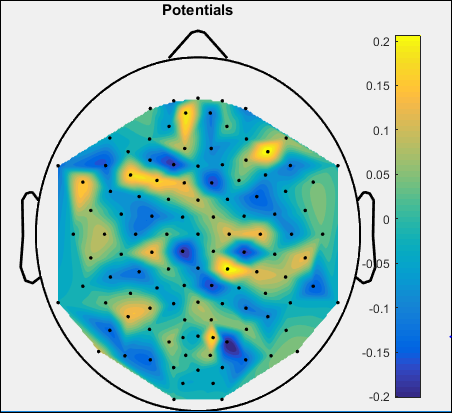
\includegraphics[keepaspectratio=true,scale=0.45]{figuras/image_csp_matlab.PNG}
	\caption{Resultados obtidos  com CSP-LDA}
	\label{resultadoLotte}
\end{figure}

Após execução do algoritmo um dos resultados apresentados na interface gráfica da ferramenta \textit{Matlab} é o tempo de execução do algoritmo de treinamento, onde obteve-se um resultado de tempo médio de processamento de aproximadamente \textbf{10.89 ms} (milissegundos).

\section{Resultados Obtidos em Linguagem C}


\section{Resultados Obtidos no Coprocessamento Hardware-Software}
As funções do algoritmo de treinamento do classificador LDA que continuaram mapeadas em software continuaram com os mesmos resultados obtidos na seção anterior. Portanto, esta seção se restringe aos resultados obtidos quanto a implementação das funções em hardware FPGA.

\subsection{Resultados Obtidos Pós Implementação em Hardware}
\subsubsection{IP Para Cálculo de Média}

Após a execução de todos os procedimentos de desenvolvimento, síntese e implementação do IP para cálculo de média, com a função de \textit{Report post-Synthesis} da ferramenta \textit{Vivado 2017.4} obteve-se os seguintes estimativas de consumo de hardware, apresentados na Tabela \ref{consumo_media}.

\begin{table}[!h]
	\centering
	\caption{Consumo de hardware da função Média.}
	\label{consumo_media}
	\begin{tabular}{ccccl}
		\textbf{}         & \textbf{LUT}  & \textbf{FF}  & \textbf{BUFG} & \textbf{DSP} \\
		\textit{Média} & \textit{40\%} & \textit{6\%} & \textit{3\%}  & \textit{1\%}
	\end{tabular}
\end{table}

A maior parte dos recursos consumidos se destinam ao somadores. Para garantir uma maior velocidade de tratamento dos dados, optou-se por não armazenar os sinais de entrada da função média em BRAMs, mas sim, lê-los diretamente dos registrados do barramento \textit{AXI-4Lite}, pois o processo de leitura e escrita nos blocos de memória RAM consomem 4 ciclos de relógio por operação. Além disso, para comando de leitura e escrita seria necessária a implementação de uma FSM o que demandaria mais recursos.\\
Os valores em porcentagem representam o consumo de acordo com as quantidades de recursos disponíveis no SoC \textit{Zynq} embarcado no kit de desenvolvimento \textit{Zybo Board 70-10} composto por uma FPGA do família \textit{Artix 7}.

\subsubsection{IP Para Cálculo da Covariância}
Utilizando-se da mesma função de ferramenta \textit{Report post-Synthesis}, obteve-se os seguintes resultados de consumo para cálculo da covariância, apresentados na Tabela \ref{consumo_cov}.

\begin{table}[!h]
	\centering
	\caption{Consumo de hardware da função Covariância.}
	\label{consumo_cov}
	\begin{tabular}{ccccl}
		\textbf{}         & \textbf{LUT}  & \textbf{FF}  & \textbf{BUFG} & \textbf{DSP} \\
		\textit{Covariância} & \textit{26\%} & \textit{5\%} & \textit{3\%}  & \textit{8\%}
	\end{tabular}
\end{table}

Grande parte do consumo de recursos da função é destinada ao processo de multiplicação e sinais de registradores para conectar os IPs de soma e multiplicação desenvolvidos por \cite{munoz2010tradeoff}.

\subsubsection{Sistema Coprocessado}

Após a integralização dos blocos IPs desenvolvidos com o SoC \textit{Zynq} e realizar a implementação do sistema geral (Anexo 01), obteve-se os seguintes resultados para consumo de recursos, apresentados na Tabela \ref{consumo_geral}

% Please add the following required packages to your document preamble:
% \usepackage[table,xcdraw]{xcolor}
% If you use beamer only pass "xcolor=table" option, i.e. \documentclass[xcolor=table]{beamer}
\begin{table}[!h]
	\centering
	\caption{Consumo de hardware do coprocessamento após implementação.}
	\label{consumo_geral}
	\begin{tabular}{lrrr}
		\rowcolor[HTML]{DAE8FC} 
		\multicolumn{1}{c}{\cellcolor[HTML]{DAE8FC}\textbf{Recursos}} & \multicolumn{1}{c}{\cellcolor[HTML]{DAE8FC}\textbf{Utilização}} & \multicolumn{1}{c}{\cellcolor[HTML]{DAE8FC}\textbf{Disponível}} & \multicolumn{1}{c}{\cellcolor[HTML]{DAE8FC}\textbf{Utilização (\%)}} \\
		LUT                                                           & 15252                                                           & 17600                                                           & 86.66                                                                \\
		\rowcolor[HTML]{DAE8FC} 
		LUTRAM                                                        & 234                                                             & 6000                                                            & 3.90                                                                 \\
		FF                                                            & 10303                                                           & 35200                                                           & 29.27                                                                \\
		\rowcolor[HTML]{DAE8FC} 
		BRAM                                                          & 6                                                               & 60                                                              & 10.00                                                                \\
		DSP                                                           & 9                                                               & 80                                                              & 11.25                                                                \\
		\rowcolor[HTML]{DAE8FC} 
		IO                                                            & 36                                                              & 100                                                             & 36.00                                                                \\
		BUFG                                                          & 4                                                               & 32                                                              & 12.00                                                                \\
		\rowcolor[HTML]{DAE8FC} 
		MMCM                                                          & 2                                                               & 2                                                               & 100.00                                                              
	\end{tabular}
\end{table}

Apesar de ainda haver insumos de hardware disponíveis optou-se por finalizar a implementação seguindo os resultados da Tabela \ref{consumo_geral}. Pois, um consumo de LUT acima de 90\% poderia resultar num mal roteamento do circuito.\\

A Figura \ref{roteamento} e a Figura \ref{legenda_rot} apresentam o roteamento do sistema de coprocessamento implementado no kit de desenvolvimento e sua legenda, respectivamente.
\begin{figure}[!h]
	\centering
	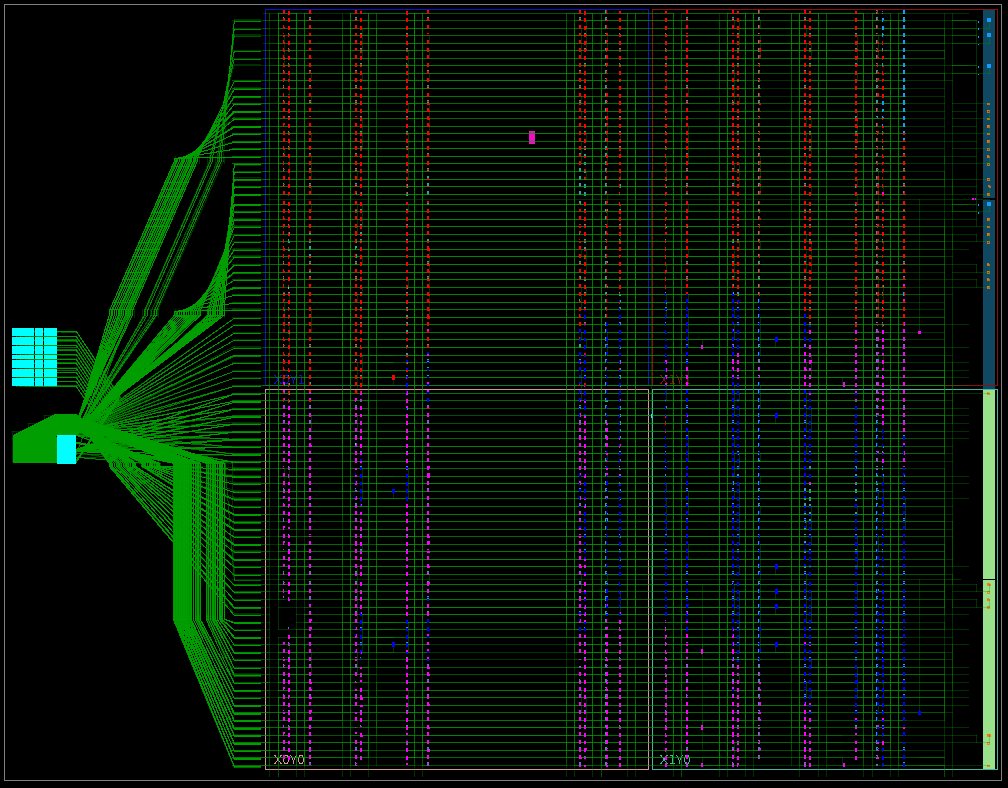
\includegraphics[keepaspectratio=true,scale=0.40]{figuras/roteamento.png}
	\caption{Roteamento do circuito implementado referente a todo o sistema de coprocessamento.}
	\label{roteamento}
\end{figure}


\begin{figure}[!h]
	\centering
	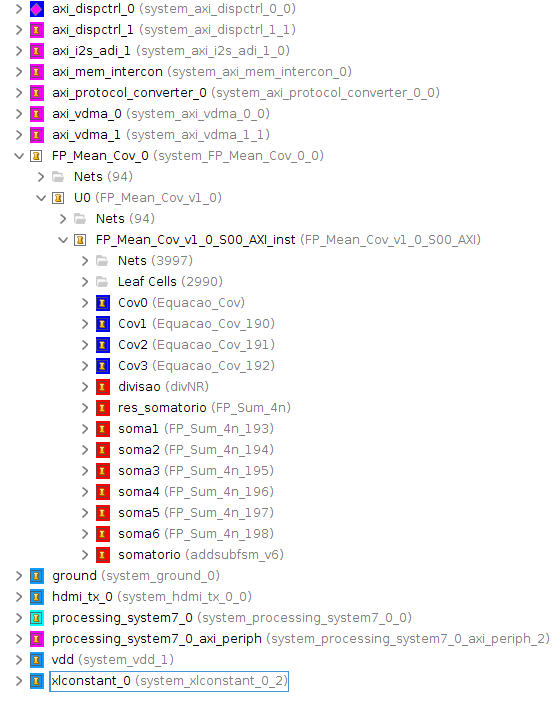
\includegraphics[keepaspectratio=true,scale=0.35]{figuras/legenda_roteamento.png}
	\caption{Legenda para a Figura \ref{roteamento}.}
	\label{legenda_rot}
\end{figure}

Os blocos em vermelho representam a alocação dos módulos pertinentes a função de cálculo de média, já se percebe que é a função que mais consumiu recursos. Em azul escuro a alocação dos módulos pertinentes a função de cálculo da covariância. Em azul turquesa a alocação dos módulos do processador \textit{ARM Cortex A9}. 
Em rosa os módulos que compõem o barramento \textit{AXI-4Lite}.\\
Uma outra informação relevante extraída pós implementação é a estimação do consumo energético de todo o sistema desenvolvido. Estas informações são fornecidas pela função \textit{report power} do \textit{Vivado}. A estimação do consumo energético é apresentado na Figura \ref{power}.
\begin{figure}[!h]
	\centering
	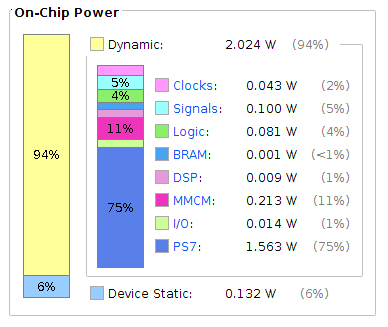
\includegraphics[keepaspectratio=true,scale=0.5]{figuras/power.png}
	\caption{Estimativa do consumo energético do sistema.}
	\label{power}
\end{figure}

A Figura \ref{power} apresenta a estimativa de consumo energético para cada componente do sistema. O processador ARM representado por PS7 na Figura \ref{power}, é o que tem maior consumo, com aproximadamente 75\% do consumo total. O sistema em geral apresentou o consumo geral de 2.156 watts.
 

\subsection{Resultados de Simulação de Hardware}
As simulações dos IPs desenvolvidos nos dá uma estimativa de desempenho de processamento dos IPs, com uma análise temporal. 

\subsubsection{IP Para Cálculo de Média}

Na plataforma \textit{Vivado 2017.4} e com um \textit{clock} estipulado em 100 MHz, a Figura \ref{simulacao_sum} apresenta a simulação temporal do IP de soma para 20 sinais de entrada.

\begin{figure}[!h]
	\centering
	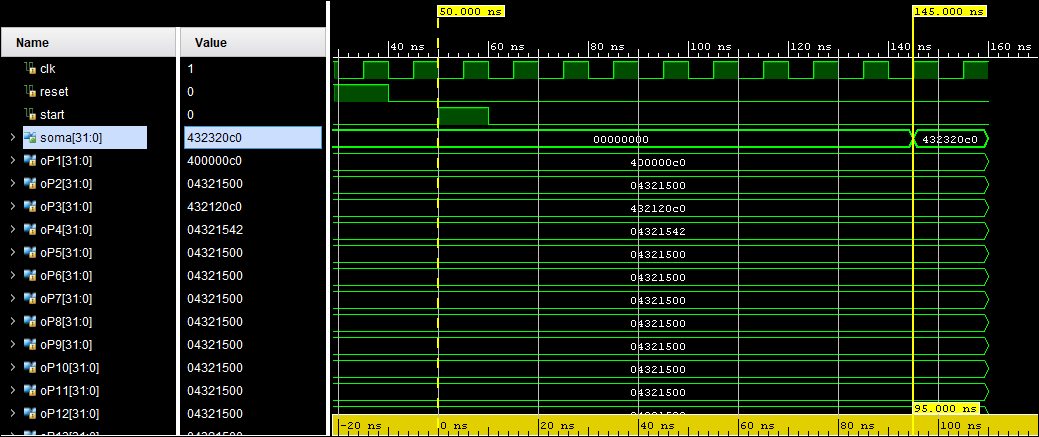
\includegraphics[keepaspectratio=true,scale=0.5]{figuras/Simulacao_somatorio.PNG}
	\caption{Simulação do IP de soma de 20 operandos.}
	\label{simulacao_sum}
\end{figure}

Na simulação (Figura \ref{simulacao_sum}), 20 valores são carregados para a entrada do somador, representados como oP1, oP2,...,oP20. O sinal de \textit{start} realiza o inicio das operações. A partir da Figura \ref{simulacao_sum} tem-se que o sinal de \textit{start} recebe nível alto no intervalo de tempo $t = 50 ns$, iniciando o processo de soma dos valores de entrada. O resultado de saída é atualizado no instante de tempo $t = 145 ns$. Ou seja, do instante de tempo que o \textit{start} é acionado ao instante em que a saída é atualizada tem-se um total de $95 ns$, isso configura o valor de \textit{latência} do hardware, ou seja, com uma $\textbf{latência = 95 ns}$, a cada sinal de \textit{start} em 95 ns é realizada uma soma de 20 operandos. Por se tratar de uma implementação em \textit{dataflow} o \textit{throughput} é igual a latência do hardware. 

Como os dados de treinamento do \textit{dataset - BCI Competition III - IVa} são matrizes de tamanho 80x6 (após a extração de características e a separação das classes), por classe, é necessária a execução do cálculo 4 vezes para somar todos os 80 dados de uma coluna de dados de uma determinada classe. O processamento em hardware retorna então para o processador ARM 1 (um) valor de soma de 20 (vinte) operandos. Como são necessária 4 somas de 20 operandos para totalizar a soma dos 80 (oitenta) amostras, os 4 (quatro) valores retornado para o ARM são retornados via AXI-Lite para o processamento em hardware, onde são somados e em seguida dividido pelo numero de amostras, resultando na média final. Como uma única soma possui \textit{throughput} = 95 ns, o somador de 4 entradas possui \textit{throughput} = 20 ns e a divisão tem \textit{troughput} = 30 ns (obtido também através da simulação do IP), pode-se obter o \textit{troughput} para cálculo da média de uma classe de acordo com a Equação \ref{eq: throughput}.

\begin{equation}
\label{eq: throughput}
	T_m = N(T_{s20}*4 + T_{s4} + T_{div})  
\end{equation}

Sendo, $T_m =$ período para cálculo da média; $N =$ número de colunas da matriz de características; $T_{s20} =$ \textit{troughput} da soma de 20 operandos; $T_{s4} =$ \textit{troughput} da soma de 4 operandos; $T_{div} =$ \textit{troughput} da divisão. Portanto para o IP de média obtemos um \textbf{$T_m = 2.58$ $\mu$s}. Ou seja, para calcular a média de cada classe será necessário um período de 2.58 $\mu$s. Como são duas classes, o período total de processamento utilizado pela função média é de \textbf{5.16 $\mu$s}.

\subsubsection{IP Para Cálculo de Covariância}

Na mesma ferramenta e mesmo \textit{clock} utilizado na simulação do IP de cálculo de média, realizou-se a simulação do IP de covariância. A Figura \ref{simulacao_cov} apresenta a simulação temporal do IP que realiza o cálculo da Equação \ref{eq: cov_hw}.


\begin{figure}[!h]
	\centering
	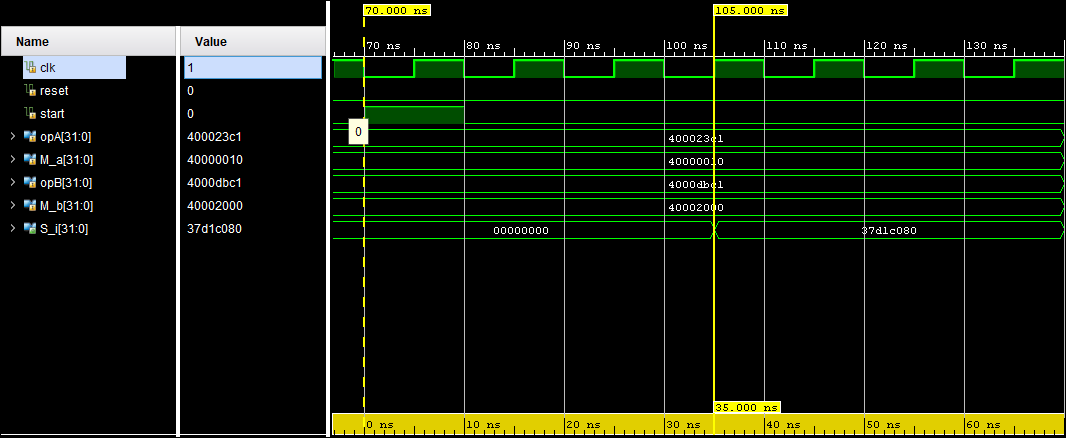
\includegraphics[keepaspectratio=true,scale=0.5]{figuras/Simulacao_cov.PNG}
	\caption{Simulação do IP de covariância para um único módulo.}
	\label{simulacao_cov}
\end{figure}

De acordo com a Figura \ref{simulacao_cov} os quatro valores necessários para o cálculo são carregados nos quatro operadores de entrada. Com o \textit{start} ativado em $t = 70 ns$ o primeiro resultado de saída é obtido em $t = 105 ns$, portanto a latência do hardware é de $t = 35 ns$, como a implementação também segue uma técnica de \textit{dataflow} este valor também é referido ao \textit{troughput} do hardware. Como são 4 implementações executando em paralelo então a cada 35 ns partindo do \textit{start} obtém-se 4 valores de saídas referente a Equação \ref{eq: cov_hw}. Como os dados de entrada se referem a uma matriz de tamanho 80x6 para cada classe, pode-se estimar o \textit{troughput} do hardware desenvolvido, a partir da Equação \ref{eq: throughput_hw}.

\begin{equation}
\label{eq: throughput_hw}
T_{cov} = \frac{N_{class}(N_{col}^2)(T_{cov1})}{N_{par}} 
\end{equation}

Sendo, $T_{cov} =$ período total de processamento da função; $N =$ número de colunas da matriz de características; $N_{class} =$ número de classes; $N_{col} =$ número de colunas da matriz de entrada; $T_{cov1} =$ \textit{troughput} da covariância, $N_{par} =$ número de implementações sendo executadas em paralelo.\\
Sendo assim, pela Equação \ref{eq: throughput_hw} tem-se que $T_{cov} =$ 50.4 $\mu$s, ou seja, o IP de cálculo em ponto flutuante da função covariância consome um tempo de processamento de 50.4 $\mu$s para calcular a covariância das duas classes dos dados de treinamento do \textit{data-set - BCI Competition III - IVa}.
\subsection{Resultados de Execução}
Após todo o processo de implementação e simulação, executou-se o sistema coprocessado utilizando-se do \textit{data-set - BCI Competition III - IVa}
como sinais de entrada, obtendo-se os seguintes resultados de acurácia apresentados na Tabela \ref{resacc}.


% Please add the following required packages to your document preamble:
% \usepackage[table,xcdraw]{xcolor}
% If you use beamer only pass "xcolor=table" option, i.e. \documentclass[xcolor=table]{beamer}
\begin{table}[!h]
	\label{resacc}
	\caption{Acurácia da classificação dos sinais com treinamento em sistema coprocessado.}
	\centering
	\begin{tabular}{lcccll}
		\rowcolor[HTML]{DAE8FC} 
		\multicolumn{1}{c}{\cellcolor[HTML]{DAE8FC}\textbf{Sistema}} & \textit{\textbf{aa}}        & \textit{\textbf{al}}        & \textit{\textbf{av}}        & \textit{\textbf{aw}} & \textit{\textbf{ay}} \\
		\textbf{Coprocessado}                                        & \multicolumn{1}{r}{65.18\%} & \multicolumn{1}{r}{96.43\%} & \multicolumn{1}{r}{50.51\%} & 59.82\%              & 57.14\%             
	\end{tabular}
\end{table}
O sistema obteve uma melhor acurácia no sujeito \textit{al}, pois é o sujeito que mais possui tarefas realizadas e préviamente classificadas. O oposto ocorre com o sujeito \textit{av}.\\
Outro dado importante coletado após a execução foi o tempo de processamento da função de treinamento implementada no sistema coprocessado. Realizando a análise de perfil, obteve-se um tempo de processamento de \textbf{10 milissegundos}.

 
\subsection{Análise de Resultados de Desempenho de Processamento}

Em cada uma das implementações foram utilizadas arquiteturas diferentes, a Tabela \ref{propriedades} apresenta as arquiteturas utilizadas em cada uma das implementações.  

% Please add the following required packages to your document preamble:
% \usepackage[table,xcdraw]{xcolor}
% If you use beamer only pass "xcolor=table" option, i.e. \documentclass[xcolor=table]{beamer}
\begin{table}[!h]
	\centering
	\caption{Propriedades das plataformas utilizadas.}
	\label{propriedades}
	\begin{tabular}{lrrr}
		\rowcolor[HTML]{DAE8FC} 
		\multicolumn{1}{c}{\cellcolor[HTML]{DAE8FC}\textbf{Implementação}} & \multicolumn{1}{c}{\cellcolor[HTML]{DAE8FC}\textbf{Sistema}} & \multicolumn{1}{c}{\cellcolor[HTML]{DAE8FC}\textbf{Processador(es)}} & \multicolumn{1}{c}{\cellcolor[HTML]{DAE8FC}\textbf{Dados}} \\
		\textit{\textbf{Matlab}}                                        & Windows 10                                                   & Intel Core i5 (2.2 GHz)                                              & 64 bits                                                    \\
		\rowcolor[HTML]{DAE8FC} 
		\textit{\textbf{Linguagem C}}                                   & Linux                                                        & ARM Cortex A9 (480 MHz)                                              & 32 bits                                                    \\
		\textit{\textbf{Hardware-Software}}                             & \textit{Zynq}                                                & ARM /Artix 7 (100 MHz)                                               & 27 bits                                                   
	\end{tabular}
\end{table}


A partir da execução de cada uma das implementações obteve-se os seguintes resultados de acurácia apresentados na Tabela \ref{acuracias}. 
% Please add the following required packages to your document preamble:
% \usepackage[table,xcdraw]{xcolor}
% If you use beamer only pass "xcolor=table" option, i.e. \documentclass[xcolor=table]{beamer}
\begin{table}[!h]
	\centering
	\caption{Acurácia das implementações de estudo.}
	\label{acuracias}
	\begin{tabular}{lccccc}
		\rowcolor[HTML]{DAE8FC} 
		\multicolumn{1}{c}{\cellcolor[HTML]{DAE8FC}\textbf{Implementação}} & \textit{\textbf{aa}} & \textit{\textbf{al}} & \textit{\textbf{av}} & \multicolumn{1}{l}{\cellcolor[HTML]{DAE8FC}\textit{\textbf{aw}}} & \multicolumn{1}{l}{\cellcolor[HTML]{DAE8FC}\textit{\textbf{ay}}} \\
		\textit{\textbf{Matlab}}                                        & 66.70\%              & 96.43\%              & 47.75\%              & 71.88\%                                                          & 49.60\%                                                          \\
		\rowcolor[HTML]{DAE8FC} 
		\textit{\textbf{Linguagem C}}                                   & 66.18\%              & 96.43\%              & 50.51\%              & 59.82\%                                                          & 57.14\%                                                             \\
		\textit{\textbf{Hardware-Software}}                             & 66.18\%              & 96.43\%              & 50.51\%              & 59.82\%                                                          & 57.14\%                                                         
	\end{tabular}
\end{table}

De acordo com a Tabela \ref{acuracias}, as implementações em linguagem C e coprocessamento obtiveram valores diferentes da implementação original em \textit{Matlab}, devido ao que apresentado na Tabela \ref{propriedades}, apresentam tamanho de dados inferiores à implementação em \textit{Matlab}. Com isso todos os sinais foram truncados em seus respectivos tamanhos de dados, propagando erros em seus cálculos em ponto flutuante.\\
Além disso a implementação em sistema coprocessado apresentou um erro quadrático médio de 0,42\% em relação à implementação \textit{Matlab}

Por se tratarem de sistemas com frequências de \textit{clock} diferentes cada uma das implementações apreseta tempos de execução diferentes. Estes tempos são apresentados na Tabela \ref{tempos}. 

% Please add the following required packages to your document preamble:
% \usepackage[table,xcdraw]{xcolor}
% If you use beamer only pass "xcolor=table" option, i.e. \documentclass[xcolor=table]{beamer}
\begin{table}[!h]
	\centering
	\caption{Tempos de execução da função de treinamento nas diferentes implementações.}
	\label{tempos}
	\begin{tabular}{lc}
		\rowcolor[HTML]{DAE8FC} 
		\multicolumn{1}{c}{\cellcolor[HTML]{DAE8FC}\textbf{Implementação}} & \textit{\textbf{Tempo de execução da função de treinamento}} \\
		\textit{\textbf{Matlab}}                                           & 10.89 ms                                                     \\
		\rowcolor[HTML]{DAE8FC} 
		\textit{\textbf{Linguagem C}}                                      & 340$\mu$s                                                 \\
		\textit{\textbf{Hardware-Software}}                                & 10 ms                                                       
	\end{tabular}
\end{table}

A implementação que obteve o melhor desempenho de processamento foi a implementação em Linguagem C embarcado no processador \textit{ARM Cortex A9} presente no \textit{SoC} do kit de desenvolvimento \textit{Zybo Board}. A implementação com menor desempenho de tempo de processamento foi a implementação em \textit{Matlab}, isto é devido o fato da implementação estar sendo executada em uma plataforma \textit{Windows 10} e por se tratar de uma linguagem de programação interpretada os outros porcessos executados juntos com a execução do algoritmo interfere em seu processamento. Já a respeito da implementação em sistema coprocessado o que se esperava era um melhor desempenho pois de acordo com os resultados obtidos em simulação os IPs de cálculos de média e de covariância apresentaram um tempo de execução extremamente baixo quando comparado com o resultado de execução obtido.
